\documentclass[a5paper,11pt]{extarticle}

\def\labauthors{Сарафанов Ф.Г., Платонова М.В.}
\def\labgroup{440}
\def\labnumber{3}
\def\labstartdate{12 марта}
\def\labtheme{Исследование биполярных процессов 
 \\[0.2em] переноса тока в
тлеющем разряде}
\def\shortlabtheme{Тлеющий разряд}

%!TEX root = ../vdiode.tex
\usepackage{cmap}
\usepackage[T2A]{fontenc}
\usepackage[utf8x]{inputenc}
\usepackage[english, russian]{babel}

\usepackage{misccorr} % в заголовках появляется точка, но при ссылке на них ее нет
\usepackage{amssymb,amsfonts,amsmath,amsthm}  
\usepackage{indentfirst}
\usepackage[usenames,dvipsnames]{color} 
\usepackage[unicode,hidelinks]{hyperref}
% \hypersetup{%
%     pdfborder = {0 0 0}
% }

\usepackage{makecell,multirow} 
\usepackage{ulem}
\usepackage{graphicx,wrapfig}
\graphicspath{{img/}}
\usepackage{geometry}
\geometry{left=1.5cm,right=1.5cm,top=2cm,bottom=2cm,bindingoffset=0cm,headheight=15pt}
\usepackage{fancyhdr} 
\linespread{1.05} 
\frenchspacing 
\renewcommand{\labelenumii}{\theenumii)} 
\newcommand{\mean}[1]{\langle#1\rangle}
% \usepackage{caption}
%%%%%%%%%%%%%%%%%%%%%%%%%%%%%%%%%%%%%%%%%%%%%%%%%%%%%%%%%%%%%%%%%%%%%%%%%%%%%%%
%%%%%%%%%%%%%%%%%%%%%%%%%%%%%%%%%%%%%%%%%%%%%%%%%%%%%%%%%%%%%%%%%%%%%%%%%%%%%%%



%%%%%%%%%%%%%%%%%%%%%%%%%%%%%%%%%%%%%%%%%%%%%%%%%%%%%%%%%%%%%%%%%%%%%%%%%%%%%%%
	%применим колонтитул к стилю страницы
\pagestyle{fancy} 
	%очистим "шапку" страницы
\fancyhead{} 
	%слева сверху на четных и справа на нечетных
\fancyhead[L]{\labauthors} 
	%справа сверху на четных и слева на нечетных
\fancyhead[R]{\shortlabtheme} 
	%очистим "подвал" страницы
\fancyfoot{} 
	% номер страницы в нижнем колинтуле в центре
\fancyfoot[C]{\thepage} 
\renewcommand{\phi}{\varphi}
%%%%%%%%%%%%%%%%%%%%%%%%%%%%%%%%%%%%%%%%%%%%%%%%%%%%%%%%%%%%%%%%%%%%%%%%%%%%%%%

\usepackage{float}
\usepackage[mode=buildnew]{standalone}
\usepackage{tikz} 
% \usepackage{subcaption}
\usepackage{csvsimple}
\usetikzlibrary{scopes}
\usetikzlibrary{%
     decorations.pathreplacing,%
     decorations.pathmorphing,%
    patterns,%
    calc,%
    scopes,%
    arrows,%
    % arrows.spaced,%
}
\makeatletter
\newif\if@gather@prefix 
\preto\place@tag@gather{% 
  \if@gather@prefix\iftagsleft@ 
    \kern-\gdisplaywidth@ 
    \rlap{\gather@prefix}% 
    \kern\gdisplaywidth@ 
  \fi\fi 
} 
\appto\place@tag@gather{% 
  \if@gather@prefix\iftagsleft@\else 
    \kern-\displaywidth 
    \rlap{\gather@prefix}% 
    \kern\displaywidth 
  \fi\fi 
  \global\@gather@prefixfalse 
} 
\preto\place@tag{% 
  \if@gather@prefix\iftagsleft@ 
    \kern-\gdisplaywidth@ 
    \rlap{\gather@prefix}% 
    \kern\displaywidth@ 
  \fi\fi 
} 
\appto\place@tag{% 
  \if@gather@prefix\iftagsleft@\else 
    \kern-\displaywidth 
    \rlap{\gather@prefix}% 
    \kern\displaywidth 
  \fi\fi 
  \global\@gather@prefixfalse 
} 
\newcommand*{\beforetext}[1]{% 
  \ifmeasuring@\else
  \gdef\gather@prefix{#1}% 
  \global\@gather@prefixtrue 
  \fi
} 
\makeatother

\usepackage{booktabs}
\usepackage{pgfplots, pgfplotstable}

\usepackage[outline]{contour}
\usepackage{tocloft}
\renewcommand{\cftsecleader}{\cftdotfill{\cftdotsep}} % for parts
% \renewcommand{\cftchapleader}{\cftdotfill{\cftdotsep}} % for chapters
\usepackage{pgfplots,pgfplotstable,booktabs,colortbl}
\pgfplotsset{compat=newest}
\usepackage{physics}
\usepackage{mathtools}
\mathtoolsset{showonlyrefs=true}
\newcommand\Smat{\hat { \mathbf { S } }}

\newcommand*\dotvec[1][1,1]{\crossproducttemp#1\relax}
\def\crossproducttemp#1,#2\relax{{\qty[\vec{#1}\times\vec{#2}\,]}}

\newcommand*\prodvec[1][1,1]{\crossproducttempa#1\relax}
\def\crossproducttempa#1,#2\relax{{\qty[{#1}\times{#2}\,]}}

% \def\E{\mathscr{E}_H}
\def\Rdim{\,\frac{\text{м}^3}{\text{А} \cdot \text{с}}}

\renewcommand{\vec}{\mathbf} % for parts
\begin{document}
%!TEX root = ../diode.tex
\begin{titlepage}
\begin{center}
% \vspace{-3em}
{\small\textsc{Нижегородский государственный университет имени Н.\,И. Лобачевского}}
\vskip 2pt \hrule \vskip 3pt
{\small\textsc{Радиофизический факультет}}

\vfill


{{\large Отчет по лабораторной работе №\labnumber}\vskip 12pt {\LARGE \bfseries \labtheme}}

	
\vspace{2cm}
{\large Работу выполнили студенты \\[-0.25em] \labgroup\  группы радиофизического факультата \\[0.5em] {\Large \bfseries \labauthors}}

% \vspace{0.5cm}
% {e-mail: sfg180@yandex.ru}

% \vspace{2cm}

\end{center}

\vfill
	
% \begin{flushright}
% 	{Выполнили студенты 430 группы\\ \labauthor}%\vskip 12pt Принял:\\ Менсов С.\,Н.}
% \end{flushright}
	
% \vfill
	
\begin{center}
	{Нижний Новгород, \labstartdate\ -- \today}
\end{center}

\end{titlepage}

\tableofcontents
\newpage



\addcontentsline{toc}{section}{Введение}
\section*{Введение}
\vspace{-0.5em}
В настоящей работе изучаются свойства \textit{тлеющего разряда}. Он принадлежит к числу самостоятельных разрядов, т.е. тлеющий разряд не гаснет после прекращения действия постороннего ионизатора и практически не нуждается в действии этого ионизатора для своего зажигания.

Тлеющий разряд, как правило, формируется при низком давлении газа и малом токе. Различают две части разряда: темное катодное пространство (несветящаяся часть, прилегающая к катоду) и положительный столб(светящийся столб газа, заполняющий остальное межэлектродное пространство). 
Причинами ионизации газа в тлеющем пространстве являются электронная эмиссия с катода (электроны соударяются с молекулами газа и ионизуют их), а также вторичная электронная эмиссия с катода, вызванная бомбардировкой катода положительно заряженными ионами газа.



\vspace{-0.5em}

\paragraph{Установка.} Установка представляет собой стеклянную трубку, заполненную инертным газом - неоном. На торцах стеклянной трубки находятся электроны, один из которых неподвижен, а другой способен перемещаться по длине трубке.
Снятие зависимости напряжения горения от межэлектродного расстояния проводилось при трех различных значениях тока, расстояние изменялось перемещением подвижного электрода вдоль трубки.
Для снятия ВАХ устанавливалось оптимальное межэлектродное расстояние, после чего снималась зависимость напряжения на электродах от тока разряда.

\newpage

% \newpage

\section{Измерения}
\subsection{Распределение потенциала}
\begin{figure}[H]
	\centering
	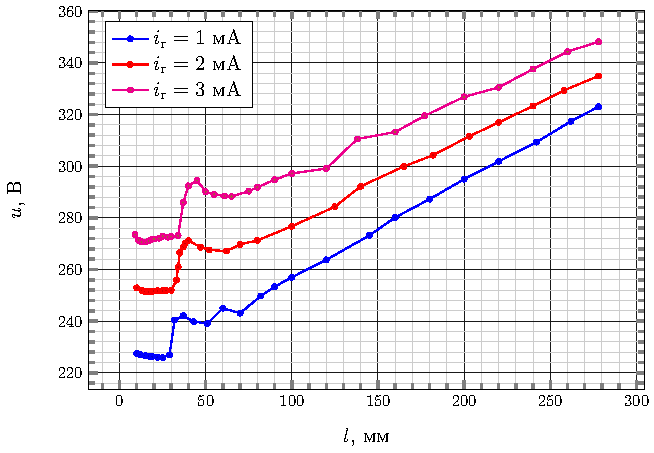
\includegraphics[]{fig/u_from_l.pdf}
	\caption{Кривые распределения потенциала}
	\label{fig:1}
\end{figure}
Из графика видно, что с увеличением тока разряда кривая распределения потенциала поднимается. То есть чем больше ток, тем при большем напряжении появляется тлеющий разряд.

Положительный столб начинается там, где зависимость потенциала от расстояния становится линейной. 
Определим катодное падение потенциала из снятых характеристик:
\begin{gather}
	i=1\text{ мА} \quad \Delta(U) = 16 \,\text{B}\\
	i=2\text{ мА} \quad \Delta(U) = 20\, \text{B}\\
	i=3\text{ мА} \quad \Delta(U) = 22 \,\text{B}
\end{gather}
Продольное падение потенциала в положительном столбе:
\begin{gather}
	i=1\text{ мА} \quad \frac{\Delta(U)}{\Delta(l)} = 4 \,\frac{\text{В}}{\text{см}}\\
	i=2\text{ мА} \quad \frac{\Delta(U)}{\Delta(l)} = 3.4\,\frac{\text{В}}{\text{см}}\\
	i=3\text{ мА} \quad \frac{\Delta(U)}{\Delta(l)} = 3 \,\frac{\text{В}}{\text{см}}
\end{gather}
Найдем, насколько уменьшится напряжение между электродами. Рассмотрим расстояния: $l=20 cm$ и $l = 5 cm$
\begin{gather}
	l=20 \,\text{см}\\
	i=1\text{ мА} \quad U = 296  \,\text{B}\\
	i=2\text{ мА} \quad U = 310  \,\text{B}\\
	i=3\text{ мА} \quad U = 327  \,\text{B}
\end{gather}
\begin{gather}
	l=5 \,\text{см}\\
	i=1\text{ мА} \quad U = 240  \,\text{B}\\
	i=2\text{ мА} \quad U = 268  \,\text{B}\\
	i=3\text{ мА} \quad U = 290  \,\text{B}
\end{gather}

Следовательно:
\begin{gather}
	i=1\text{ мА} \quad \Delta(U) = 56  \,\text{B}\\
	i=2\text{ мА} \quad \Delta(U) = 42  \,\text{B}\\
	i=3\text{ мА} \quad \Delta(U) = 37  \,\text{B}
\end{gather}
При повышении тока падение потенциала в положительном столбе уменьшается.
\subsection{ВАХ тлеющего разряда}
\begin{figure}[H]
	\centering
	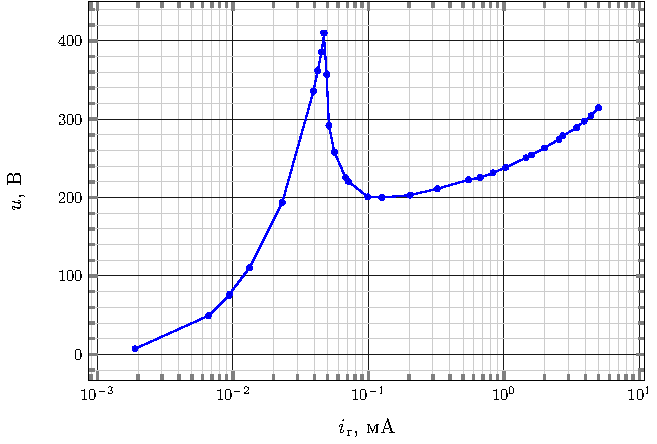
\includegraphics[]{fig/vax.pdf}
	\caption{Вольт-амперная характеристика тлеющего разряда}
	\label{fig:2}
\end{figure}
Второго пика достичь не удалось, так как ток в установке не должен превышать $5\text{ мА}$.


\addcontentsline{toc}{section}{Заключение}
\section*{Заключение}
В настоящей работе мы изучили процессы переноса тока в тлеющем разряде, сняли ВАХ разряда, а так же зависимость напряжения разряда от расстояния между анодом и катодом.

% \begin{thebibliography}{}
%   \bibitem{orlov} Орлов И.\,Я., Односевцев В.\,А. и др. Основы радиоэлектроники: учебное пособие. -- Нижний Новгород: Нижегородский государственный университет им. Н.И. Лобачевского, 2011. -- 169 с.
  
%   \bibitem{met} Битюрин\,\,Ю.\,А. и др. Измерение статических характеристик полупроводникового диода. Н.Новгород: ННГУ, 2004. -- 38 с.
  
%   % \bibitem{lit3} Ландау Л.Д., Лифшиц Е.М. Любой том. М.: Физматлит, 2003.
% \end{thebibliography}

\end{document}